\chapter{Revisão Bibliográfica}

No presente capítulo, são apresentados conceitos básico para a compreensão do trabalho. Nessa etapa, busca-se através da revisão de trabalhos já elucidados a contextualização do projeto proposto.


%%%%%%%%%%%%%%%%%%%%%%%%%%%%%%%%%%%%%%%%%%%%%%%%%%%%%%%%%%%%%%%%%%%%%%

\section{Satélites Artificiais} %ch 1303

Desde o lançamento do satélite Sputnik I, primeiro satélite artificial, que foi desenvolvido e lançado pela extinta URSS (União das Repúblicas Socialistas Soviéticas) no dia 4 de Outubro de 1957, novas formas de controle foram desenvolvidas. Como o principal fim de um satélite é a comunicação e a navegação, que exigem orientação acurada, juntamente com todas as forças que atuam sobre o satélite, se torna imprescindível o uso de técnicas de controle para se garantir a translação e a rotação do satélite \cite{Brown2002}. Na figura \ref{fig:rotational_brown_p256}, podemos ver os movimentos de rotação e translação de um satélite ao redor de um planeta.

\begin{figure}[H]
  \caption{Movimento de translação de um satélite artificial.}
  \begin{center}
      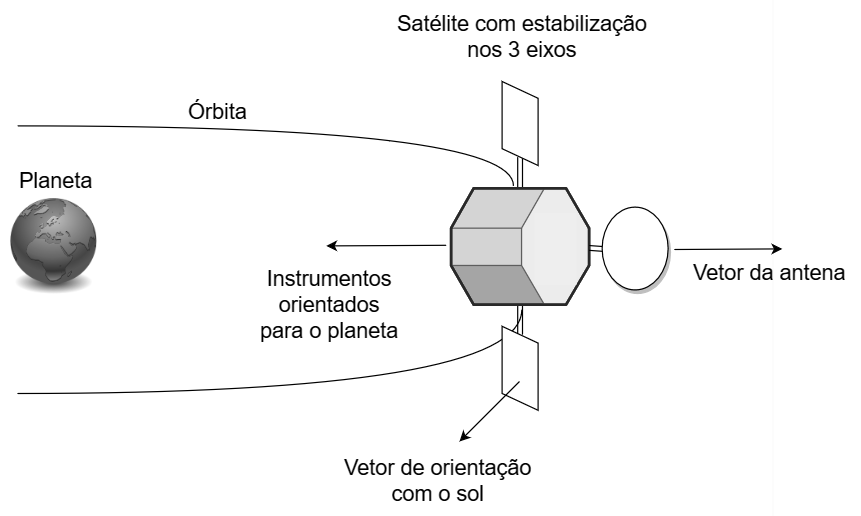
\includegraphics[scale=0.5]{referencial/img/rotational_brown_p256}
  \end{center}
  \fonte{Adaptado de \citeonline{Brown2002}.} 
  \label{fig:rotational_brown_p256}
\end{figure}

A dinâmica de rotação é descrita no próximo item, juntamente com todas as ferramentas matemáticas para sua modelagem. 

%%%%%%%%%%%%%%%%%%%%%%%%%%%%%%%%%%%

\subsection{Dinâmica de um Satélite}\label{cap:dinamica}

A dinâmica é dividida em duas partes, onde uma representa os movimentos de translação e a outra os de rotação. A \textit{dinâmica de translação} de um copo em relação ao outro é um caso de \textit{Dinâmica de Corpo Rígido}. A fundação da Dinâmica de corpos rígidos foi feita pelo Físico Inglês Isaac Newton em forma de três leis, das quais, a 2º e a 3ª são primordiais para descrever a \textit{dinâmica de rotação} \cite{Snider}. A 2ª lei de Newton pode ser escrita das seguintes forma:

\begin{equation}\label{eq:fma}
  \vec{F}=\frac{d}{dt}\vec{p}\quad\quad\quad\quad\vec{p}=m\vec{v}
\end{equation}

\begin{equation}
  \vec{F}=m\vec{a}
\end{equation}

Onde $\vec{F}$ é a força, $\vec{p}$ é o momento linear, $\vec{v}$ é a velocidade e $\vec{a}$ é  aceleração. Ainda, podemos descrever a força total sobre uma partícula $\vec{F}_i$ da seguinte forma:

\begin{equation}\label{eq:Fi}
\vec{F}_i=\vec{f}_{ie}+\sum_{i\neq j}^{N}{\vec{f}_{ie}} = m_i\vec{a}_i
\end{equation}
 
 Onde, $\vec{f}_{ie}$ é a força externa e $\vec{f}_{ij}$ é a força interna de carda parte j que compõe o corpo i e $m_i\vec{a}_i$ é a massa e a força resultante no corpo rígido. Ao unirmos N partículas para formar um corpo rígido, estamos somando todas as forças externas e as forças internas de todos os corpos da seguinte forma:

\begin{equation}
  \sum_{i=1}^{N}{\vec{F}_i}=\sum_{i=1}^{N}{\vec{f}_i}+\sum_{i=1}^{N}{\sum_{i\neq j}^{N}{\vec{f}_ij=}}\sum_{i=1}^{N}{m_i\vec{a}_i} 
\end{equation}

Segundo a 3ª Lei de Newton, como o corpo j exerce uma força $\vec{f}_{ji}$ em módulo igual a força $\vec{f}_{ij}$ que o corpo i exerce sobre o corpo j, só que oposta. Logo, as forças internas se anulam. Quando temos um conjunto de partículas unidas, podemos descrever a força total sobre o corpo ($\vec{F}_e$) como o somatório de todas as forças sobre as partículas ($\vec{F}_{ie}$). Isso pode ser escrito da seguinte forma:

\begin{equation}\label{eq:fet}
  \vec{F}_{e}=\sum_{i=1}^{N}{\vec{f}_{ie}}=\sum_{i=1}^{N}{m_i\vec{a}_i} 
\end{equation}

A imagem \ref{fig:translacao_referencial_snider_p15}, representa o vetor posição $\vec{r_{com}}$ de um corpo rígido em relação a origem. A descrição matemática desse vetor pode ser visto na equação \ref{eq:rcom}.

\begin{figure}[H]
  \caption{Representação de $\vec{r}_{com}$}
  \begin{center}
      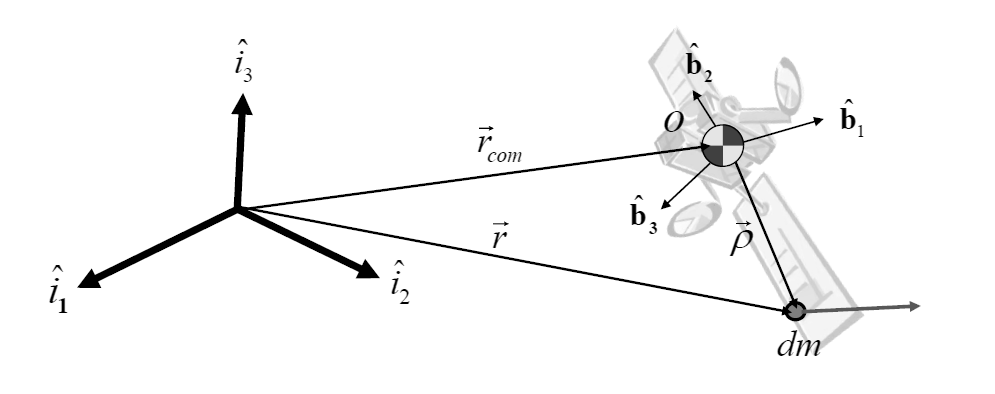
\includegraphics[scale=0.5]{referencial/img/translacao_referencial_snider_p15}
  \end{center}
  \fonte{Adaptado de \citeonline{Snider}.} 
  \label{fig:translacao_referencial_snider_p15}
\end{figure}

\begin{equation}\label{eq:rcom}
  \vec{r}_{com}=\frac{1}{M_T}\sum_{i=1}^{N}{m_i\vec{r}_i} 
\end{equation}

Onde, $M_T$ é a massa total do corpo rígido.

Como a aceleração é a derivada segunda da posição, derivamos duas vezes a posição $\vec{r}_{com}$ e multiplicamos pela massa total em ambos os lado da equação \ref{eq:rcom}. Assim temos:

\begin{equation}\label{eq:2deriv}
  M_T\frac{{d}^{2}}{{d}t^{2}}\vec{r}_{com}=\sum_{i=1}^{N}{m_i\vec{a_i}}
\end{equation}

Igualando as equações \ref{eq:fet} e \ref{eq:2deriv}, temos a força total sobre um corpo rígido que desempenha movimento de translação. Isso pode ser visto na sequência.

\begin{equation}
\vec{F_e}=M_{T}\frac{{d}^{2}}{{d}t^{2}}\vec{r}_{com}
\end{equation}

A \textit{dinâmica de rotação} descreve o movimento de um corpo rígido em relação a um ponto. Para descrevermos os movimentos de rotação, devemos conhecer a distribuição de massa do corpo rígido \cite{Snider}. A figura \ref{fig:mass_snider_p16} ilustra a distribuição de massa infinitesimal de um corpo tridimensional. Por definição, o momento de inércia infinitesimal disposto sobre um eixo ($I_{xx}$, $I_{yy}$ e $I_{zz}$) é o produto da massa pela distância do ponto de referência. Se fizermos isso para N partículas, temos:

\begin{figure}[H]
  \caption{Distribuição de massa.}
  \begin{center}
      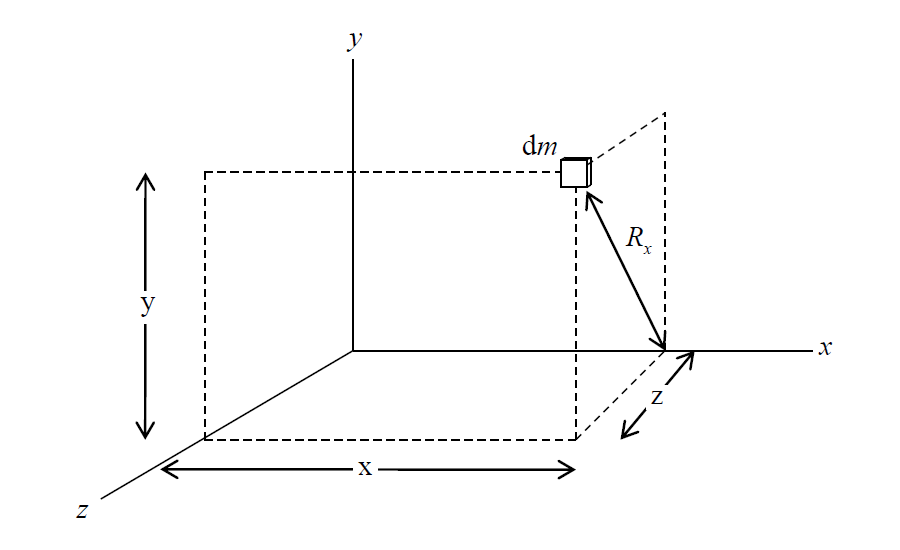
\includegraphics[scale=0.5]{referencial/img/mass_snider_p16}
  \end{center}
  \fonte{Adaptado de \citeonline{Snider}.} 
  \label{fig:mass_snider_p16}
\end{figure}

\begin{equation}
  I_{xx}=\sum_{i=1}^{N}{m_i({y_i}^{2}+{z_i}^{2})}
\end{equation}

\begin{equation}
  I_{yy}=\sum_{i=1}^{N}{m_i({x_i}^{2}+{z_i}^{2})}
\end{equation}

\begin{equation}
  I_{zz}=\sum_{i=1}^{N}{m_i({x_i}^{2}+{y_i}^{2})}
\end{equation}

Já quando as partículas estão dispostas sobre os planos xy, xz e yz, temos:

\begin{equation}
  I_{xy}=-\sum_{i=1}^{N}{m_ix_iy_i}=I_{xy}
\end{equation}

\begin{equation}
  I_{xz}=-\sum_{i=1}^{N}{m_ix_iz_i}=I_{zx}
\end{equation}

\begin{equation}
  I_{yz}=-\sum_{i=1}^{N}{m_iy_iz_i}=I_{zy}
\end{equation}

Com isso, podemos criar uma matriz que representa o momento de inércia total do corpo rígido:

\begin{equation}\label{eq:nsimetrico}
I=\begin{bmatrix}I_{xx}&I_{xy}&I_{xz}\\I_{yx}&I_{yy}&I_{yz}\\I_{zx}&I_{zy}&I_{zz}\end{bmatrix}
\end{equation}

Caso o satélite seja simétrico, os momentos de inércia nos planos xy, xz e yz são de mesmo módulo só que com sinal oposto aos momentos de inércia dos planos xy, zx e zy, anulando todos esses termos. Isso pode ser visto na seguinte matriz diagonal:

\begin{equation}
I=\begin{bmatrix} I_{ xx } & 0 & 0 \\ 0 & I_{ yy } & 0 \\ 0 & 0 & I_{ zz } \end{bmatrix}=\begin{bmatrix} A & 0 & 0 \\ 0 & B & 0 \\ 0 & 0 & C \end{bmatrix}
\end{equation}

Para facilitar a escrita das equações, os momentos de inércia $I_{xx}$, $I_{yy}$ e $I_{zz}$ serão descritos como A, B e C respectivamente. Após a descrição matemática do momento de inércia, podemos começar a analisar o movimento de rotação do corpo rígido. Vamos começar pela velocidade angular instantânea $\omega$, que pode ser descrita como a derivada primeira da posição $\beta$ angular, segundo o teorema fundamental do cálculo:

\begin{equation}
\omega\equiv\lim_{\Delta t\rightarrow 0}\frac{\Delta\beta}{\Delta t}=\frac{d\beta}{dt}
\end{equation}

A aceleração angular $\alpha$, nada mais é do que a primeira derivada da velocidade angular:

\begin{equation}
\alpha\equiv\lim_{\Delta t\rightarrow 0}\frac{\Delta\omega}{\Delta t}=\frac{d\omega}{dt}
\end{equation}

Outra equação importante para descrever a maioria dos tipos de movimento, é aquela que relaciona a posição $\beta$ com a posição inicial $\beta_0$, velocidade angular inicial $\omega_0$, o tempo inicial do movimento $t_0$, o tempo atual t e a aceleração angular $\alpha$. A expressão pode ser vista na sequência.

\begin{equation}
\beta=\beta_{0}+\omega_{0}(t-t_{0})+\frac{1}{2}\alpha{(t-t_{0})}^{2}
\end{equation}

Não menos importante, é a expressão que relaciona a velocidade angular $\omega$ com a velocidade angular inicial $\omega_0$, aceleração angular e o deslocamento ($\beta-\beta_0$). Isso é descrito na equação da sequência.

\begin{equation}
{\omega}^{2}={\omega_0}^{2}+2\alpha(\beta-\beta_0) 
\end{equation}

Como foi feito na dinâmica de translação, precisamos relacionar os momentos e a aceleração angular $\alpha$. Para isso vamos começar relacionando o torque $\vec{\tau}$ com a derivada do momento angular $\vec{L}$:

\begin{equation}
\vec{\tau}=\dot{\vec{L}}
\end{equation}

Mas como o momento angular é o produto do momento de inércia do corpo I pela velocidade angular, assim: 

\begin{equation}\label{eq:iomega}
\vec{L}=I\vec{\omega}
\end{equation}

Com isso, já conhecendo as relações entre velocidade e aceleração, temos:  

\begin{equation}\label{iomega}
\vec{\tau}=I\dot{\vec{\omega}}=I\vec{\alpha}
\end{equation}

Se usarmos o teorema do transporte cinemático, o momento de inércia pode ser escrito da seguinte forma:

\begin{equation}
\dot{\vec{L}}=I\dot{\vec{\omega}}+\vec{\omega}\times I \vec{\omega}
\end{equation}

Por consequência, descrevemos o torque da seguinte maneira:

\begin{equation}\label{eq:torque}
\vec{\tau}=I\dot{\vec{\omega}}+\vec{\omega}\times I \vec{\omega}
\end{equation}

Como temos o momento de inércia do corpo rígido representado em forma de matriz, precisamos mudar a representação a matricial. Começaremos pela velocidade angular $\vec{\omega}$, que em módulo, pode ser descrita da seguinte forma:

\begin{equation}
\left|\vec{\omega}\right|=\begin{bmatrix}\omega_1\\\omega_2\\\omega_2\end{bmatrix}
\end{equation}

Se fizermos o mesmo com a equação \ref{eq:torque}, temos:

\begin{equation}
\begin{bmatrix}\tau_{1}\\\tau_{2}\\\tau_{3}\end{bmatrix}=\begin{bmatrix}A\dot{\omega}_{1}\\B\dot{\omega}_{2}\\C\dot{\omega}_{3}\end{bmatrix}+\begin{bmatrix}\omega_{1}\\\omega_{2}\\\omega_{3}\end{bmatrix}\times\begin{bmatrix}A\omega_{1}\\B\omega_{2}\\C\omega_{3}\end{bmatrix}
\end{equation}

Como podemos ver, já conseguimos relacionar os momentos de inércia do corpo rígido simétrico com as demais variáveis de interesse. Além disso, podemos sair da forma matricial e apresentarmos os torques da forma algébrica, isso pode ser visto nas 3 equações a seguir.

\begin{equation}
  \tau_1=A\dot{\omega_1}-(B-C)\omega_2\omega_3 
\end{equation}

\begin{equation}
  \tau_2=B\dot{\omega_2}-(C-A)\omega_1\omega_3 
\end{equation}

\begin{equation}
  \tau_3=C\dot{\omega_3}-(A-B)\omega_1\omega_2
\end{equation}

Se utilizarmos um corpo não simétrico, podemos recorrer a matriz da equação \ref{eq:nsimetrico}, e obteremos as 3 seguintes equações para descrever o torque:

\begin{equation}\label{eq:torquexyz}
 \tau_{1}=I_{xx}\dot{\omega_{1}}-I_{xy}(\dot{\omega_{2}}-\omega_{1}\omega_{3})-I_{xz}(\dot{\omega_{3}}+\omega_{1}\omega_{2})\\-(I_{yy}-I_{zz})\omega_{2}\omega_{3}-I_{yz}({\omega_{2}}^{2}-{\omega_{3}}^{2})
\end{equation}

\begin{equation}\label{eq:torquexyz2}
  \tau_{2}=I_{zz}\dot{\omega_{3}}-I_{yz}(\dot{\omega_{3}}-\omega_{1}\omega_{2})-I_{xy}(\dot{\omega_{1}}+\omega_{2}\omega_{3})\\-(I_{zz}-I_{xx})\omega_{1}\omega_{3}-I_{xz}({\omega_{3}}^{2}-{\omega_{1}}^{2})
\end{equation}

\begin{equation}\label{eq:torquexyz3}
 \tau_{3}=I_{zz}\dot{\omega_{1}}-I_{xz}(\dot{\omega_{1}}-\omega_{2}\omega_{3})-I_{yz}(\dot{\omega_{2}}+\omega_{1}\omega_{3})\\-(I_{xx}-I_{yy})\omega_{1}\omega_{2}-I_{xy}({\omega_{1}}^{2}-{\omega_{2}}^{2})
\end{equation}

Se isolarmos a derivada da velocidade angular na nas equações \ref{eq:torquexyz}, \ref{eq:torquexyz2} e \ref{eq:torquexyz3}, temos:

\begin{equation}
  \dot{\omega_{1}}=\frac{\tau_{1}}{A}+\left(\frac{B-C}{A}\right)\omega_{2}\omega_{3}
\end{equation}

\begin{equation}
  \dot{\omega_{2}}=\frac{\tau_{2}}{B}+\left(\frac{C-A}{B}\right)\omega_{1}\omega_{3}
\end{equation},

\begin{equation}
  \dot{\omega_{3}}=\frac{\tau_{2}}{C}+\left(\frac{A-B}{C}\right)\omega_{1}\omega_{2}
\end{equation}

Assim conseguimos a relação da velocidade com o torque aplicado. Essa é uma expressão que representa a reação em forma de variação de velocidade que um torque provoca.


%%%%%%%%%%%%%%%%%%%%%%%%%%%%%

\subsubsection{Rodas de Reação}

Uma roda de reação consiste em um dispositivo que é fixado em um eixo de motor, com o objetivo de interferir na posição de um corpo através da variação de velocidade angular das rodas. Quando a roda sofre uma variação da sua velocidade angular, ela exerce um torque em uma determinada direção \cite{BongWie2001}. Esse efeito ocorre devido à conservação do momento angular do corpo, logo, se a roda está sendo desacelerada, o corpo tende se opor a esse movimento. Na figura \ref{fig:satellite_controlhand_p1306} podemos ver 3 rodas de reação dispostas nos 3 eixos de um corpo rígido.

\begin{figure}[H]
  \caption{Representação simplificada de um corpo rígido com rodas de reação.}
  \begin{center}
      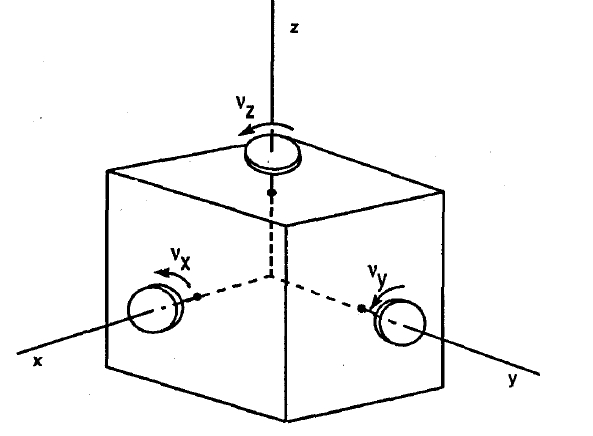
\includegraphics[scale=0.65]{referencial/img/satellite_controlhand_p1306}
  \end{center}
  \fonte{Adaptado de \citeonline{Levine1996}.} 
  \label{fig:satellite_controlhand_p1306}
\end{figure}

Como já foram descritos nas outras seções, precisamos encontrar uma relação que expresse o torque criado pelas rodas de reação, para que consigamos unir ao modelo do satélite. Para isso, começamos pelo momento angular total $\vec{L}_{total}$, que pode ser visto na sequência:

\begin{equation}\label{eq:ltot}
\vec{L}_{total}=\vec{L}_s+\vec{L}_{\omega}=constante 
\end{equation}

Onde $L_s$ representa o momento angular do satélite e $\vec{L}_{\omega}$ o momento angular da roda de reação. Como já vimos na equação \ref{eq:iomega}, o momento angular pode ser descrito da seguinte forma:

\begin{equation}
\vec{L}_s=I\vec{\omega}
\end{equation}

E o momento angular nas rodas de ração pode ser escritos da seguinte forma:

\begin{equation}
\vec {L}_{\omega} =J_{\omega}\vec{\psi}_{\omega}
\end{equation}

Onde $J_{\omega}$ é o momento de inércia da roda de reação e $\vec{\psi}_{\omega}$ é variação instantânea da posição angular da roda. Com isso, conseguimos encontrar o torque provido pela roda de reação $\tau_{\omega}$:

\begin{equation}\label{eq:torqueedo}
\vec{\tau}_{\omega}=\dot{\vec{L}}_{\omega}=J_{\omega}\dot{\vec{\psi}}_{\omega}
\end{equation}

E por fim, podemos relacionar as velocidades angulares do satélite com o as inércia e as velocidades das rodas da seguinte forma:

\begin{equation}\label{eq:modeloA}
  \dot{\omega_{1}}=\frac{J_{\omega 1}\dot{\vec{\psi}}_{\omega 1}}{A}+\left(\frac{B-C}{A}\right)\omega_{2}\omega_{3}
\end{equation}

\begin{equation}\label{eq:modeloB}
  \dot{\omega_{2}}=\frac{J_{\omega 2}\dot{\vec{\psi}}_{\omega 2}}{B}+\left(\frac{C-A}{B}\right)\omega_{1}\omega_{3}
\end{equation},

\begin{equation}\label{eq:modeloC}
  \dot{\omega_{3}}=\frac{J_{\omega 3}\dot{\vec{\psi}}_{\omega 3}}{C}+\left(\frac{A-B}{C}\right)\omega_{1}\omega_{2}
\end{equation}

Para isso é usada a equação \ref{eq:ltot} e a relação entre torque e momento angular da equação \ref{eq:torqueedo}. Assim, temos a última equação que faltava para descrever toda a dinâmica de um satélite artificial simétrico. 


%%%%%%%%%%%%%%%%%%%%%%%%%%%%%%%%%%%%%%%%%%%%%%%%%%%%%%%%%%%%%%%%%%%%%%

\section{Controladores PID}

Como já temos as equações diferenciais que descrevem o modelo satélite, precisamos desenvolver os conceitos básicos de controle para controlarmos as variáveis de interesse. Esses conceitos estão descritos nas próximas seções


%%%%%%%%%%%%%%%%%%%%%%%%%%%%%%%%%%%

\subsection{Resposta ao Degrau do um Sistema}

Um problema fundamental em engenharia, é prever e modelar sistemas naturais ou artificias para tirarmos o melhor proveito de suas características. Para isso, muitas técnicas foram desenvolvidas para se conseguir controlar essas variáveis de interesse \cite{Levine1996}. Uma forma clássica de representar uma resposta de uma variável de interesse, é através da resposta ao degrau. Essa pode ser vista na figura \ref{fig:transient_ogata_p170}, onde temos as principais características da resposta ao degrau de um sistema de segunda ordem ou superior. Onde \textit{$M_p$} (maximum overshoot) é o sobressinal da variável de interesse em percentual, \textit{$t_d$} (Delay Time) é o tempo atraso de transporte, \textit{$t_r$} (rise time) é o tempo necessário para atingir o valor do sinal de referência, \textit{$t_p$} é o tempo de pico (peak time) e \textit{$t_s$} (settling time) é o tempo para o sistema entrar em regime, observando um critério de erro em regime \cite{Ogata}.

\begin{figure}[H]
  \caption{Parâmetros de uma resposta ao degrau de um sistema de segunda ordem ou superior.}
  \begin{center}
      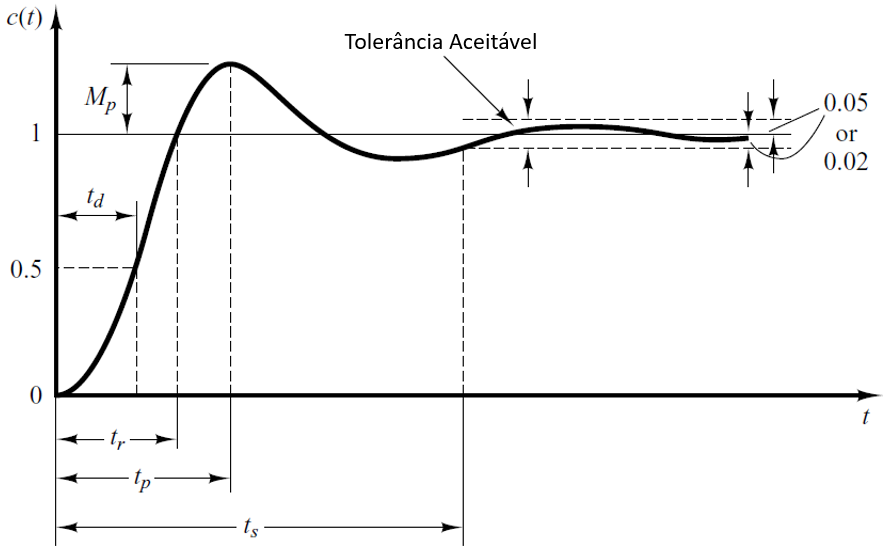
\includegraphics[scale=0.5]{referencial/img/transient_ogata_p170}
  \end{center}
  \fonte{Adaptado de \citeonline{Ogata}.} 
  \label{fig:transient_ogata_p170}
\end{figure}

A resposta ao degrau nos diz muito sobre os sistemas de interesse, pois nela podemos ver claramente a atuação dos \textit{polos} e \textit{zeros} dominantes e o ganho de baixa frequência da função de transferência do sistema. Os métodos clássicos para se calcular os parâmetros de controladores são baseados na resposta ao degrau \cite{Ogata}. 


%%%%%%%%%%%%%%%%%%%%%%%%%%%%%%%%%%%

\subsection{Controlador PID}

O controlador proporcional-integral-derivativo é um dos controladores mais utilizados nas aplicações industriais. Essa topologia de controlador consegue, em diferentes configurações atender entre 90 e 95\% de todos os sistemas que necessitam de controladores \cite{Levine1996}. A forma descritiva matemática mais comum de se encontrar um controlador PID no domínio do tempo é a seguinte:

\begin{equation}\label{eq:PID}
  u(t) = K\left((e(t)+\frac{1}{T_i}\int_{0}^{t}{e(\tau)}d\tau+T_d\frac{de(t)}{dt}\right) 
\end{equation}

Onde \textit{e(t)} é o erro, \textit{$T_i$} é o tempo integral, \textit{$T_d$} é o tempo derivativo e \textit{K} o ganho proporcional. Uma outra forma de se representar os tempos integral e derivativo, é através dos ganhos \textit{$K_i$} que é o ganho integral e o \textit{$K_d$}, que é o ganho derivativo \cite{Astrom1995}.s

Na figura \ref{fig:pid_controller_Snider_p35}, podemos ver a configuração mais utilizada do controlador PID, onde $\beta_{com}(S)$ é o valor do sinal de referência no domínio da frequência, \textit{err(S)} o erro, \textit{$K_p$} é o ganho proporcional, \textit{$K_i$} é o ganho integral, \textit{$K_d$} é o ganho derivativo, \textit{D(S)} é um distúrbio, \textit{$G_p(S)$} é a função de transferência da planta e por fim, \textit{$\beta(S)$} que é a variável de interesse \cite{Snider}.

\begin{figure}[H]
  \caption{Representação do modelo paralelo de um controlador PID com distúrbios.}
  \begin{center}
      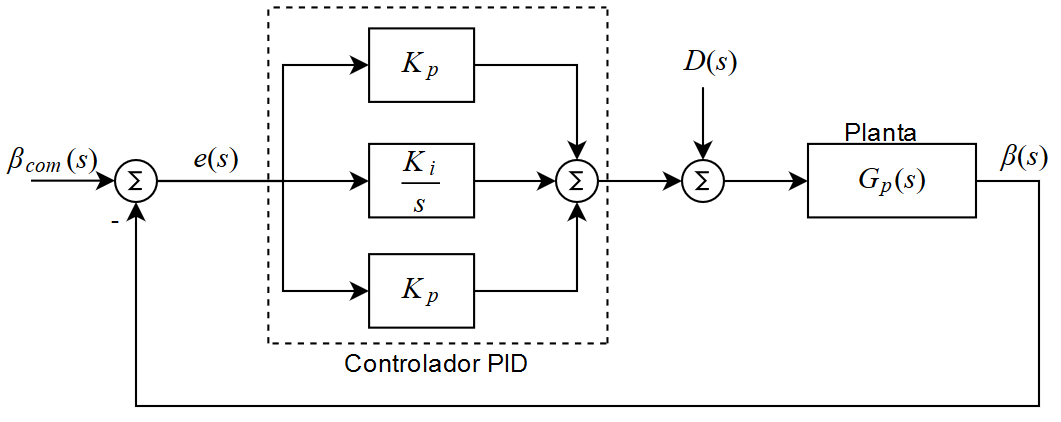
\includegraphics[scale=0.55]{referencial/img/pid_controller_Snider_p35}
  \end{center}
  \fonte{Adaptado de \citeonline{Snider}.} 
  \label{fig:pid_controller_Snider_p35}
\end{figure}

Como alguns sistemas podem admitir grandes e rápidas variações de sinais de referência, exigindo uma grande força de controle e energia no atuador, algumas topologias foram desenvolvidas para limitar a atuação de alguns fatores dos controladores. Um bom exemplo é o \textit{anti-windup}, onde essa topologia limita a saturação do atuador quando o sistema atinge o regime, causado pela ação integral. Essa topologia pode ser vista no modelo da figura \ref{fig:pid_antiwindup_astrom_p83} \cite{Astrom1995}.

\begin{figure}[H]
  \caption{Modelo de um controlador PID com histerese.}
  \begin{center}
      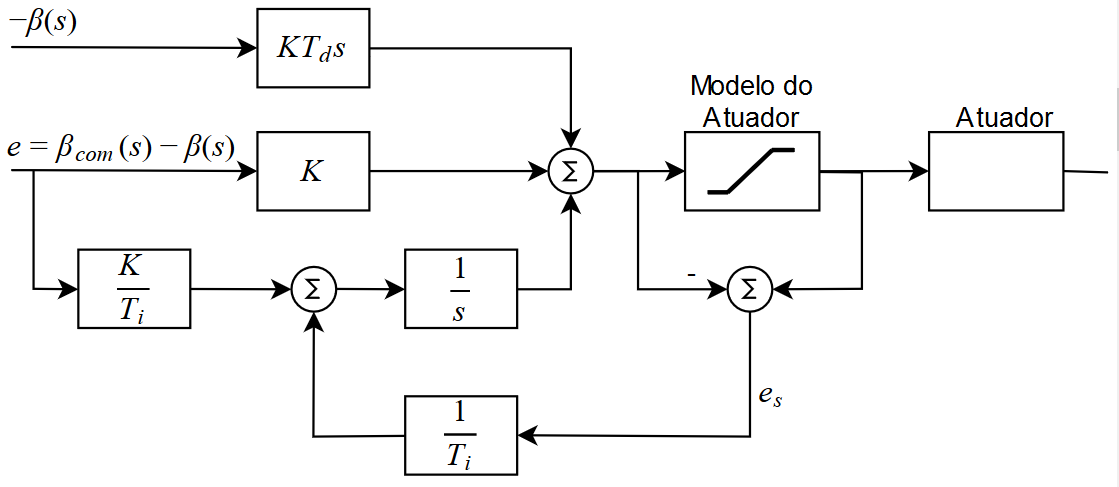
\includegraphics[scale=0.55]{referencial/img/pid_antiwindup_astrom_p83}
  \end{center}
  \fonte{Adaptado de \citeonline{Astrom1995}.} 
  \label{fig:pid_antiwindup_astrom_p83}
\end{figure}

Existem muitas combinações de controladores PID, cada uma com suas peculiaridades e vantagens de uso. Uma combinação muito usada é a PI, onde a acão integral de zerar o erro em regime e uma boa resposta transitória já satisfazem as especificações. 


%%%%%%%%%%%%%%%%%%%%%%%%%%%%%%%%%%%

\subsection{Controle Digital}

Quando utilizamos um dispositivo digital como controlador, temos que representar os sinais de forma discretizada, ou seja, em níveis que possam ser transformados em um conjunto de bits. Só assim o microcontrolador ou microprocessador poderá realizar as operações matemáticas desejadas. Para essa transformação, usamos coversores AD (analógico-digital) que convertem um sinal analógico (contínuo) em um sinal binário \cite{BongWie2001}. Um sinal analógico é representado digitalmente com um período T, da seguinte forma:

\begin{equation}
  y(0), y(T), y(2T), ...
\end{equation}

Se expressarmos usando notação ${y[kT]}$, podemos representar uma equação diferencial da seguinte forma:

\begin{equation}
  u(k) = a_{0}y[k]+a_{1}y[k-1]+...+a_{n}y[k-n] - b_{1}y[k-1] - b_{2}y[k-2] - ... -b_{n}y[k-n]
\end{equation}

Onde u(k) denota o sinal computado e y(k) os valores o sinal analógico nos instante k-ésimos.


%%%%%%%%%%%%%%%%%%%%%%%%%%%%%%%%%%%

\subsubsection{Transformada Z}

A transformada z é usada para aquisição e processamento de dados em sistemas discretos. Ela possui relação matemática com o domínio s da seguinte forma:

\begin{equation}
Z = e^{-Ts}
\end{equation}

Por definição, a transformada z é um somatório do produto de $z^{-k}$ com o valor do sinal analógico amostrado no momento k, y(k). Isso pode ser conferido na equação as seguir.

\begin{equation}
  y(z) \sum_{k=0}^{\infty}{y[k]z^{-k}} = y[0] + y[1]z^{-1}+y[2]z^{-2}...
 \end{equation} 

 Se usarmos os Teoremas da Tradução, Valor Inicial e Valor Final, conseguimos expressar uma função da seguinte forma \cite{BongWie2001}:

\begin{equation}
  \frac{u(z)}{y(z)} = \frac{a_0 + a_1z^{-1}+...+a_nz^{-n}}{1+b_1z^{-1}+b_2z^{-2}+...++b_nz^{-n}}
\end{equation}


%%%%%%%%%%%%%%%%%%%%%%%%%%%%%%%%%%%

\subsubsection{Amostragem}

Em um sistema discreto, uma forma de amostrar um sinal analógico é usar um trem de impulsos com amplitude do sinal y(t) nos tempos T e reter esses dados com um ZOH (Zero-Order-Hold - Amostrador de Ordem Zero). A figura \ref{fig:zoh_wie_p155} representa muito bem esse processo.

\begin{figure}[H]
  \caption{Conversão de um sinal contínuo em discreto.}
  \begin{center}
      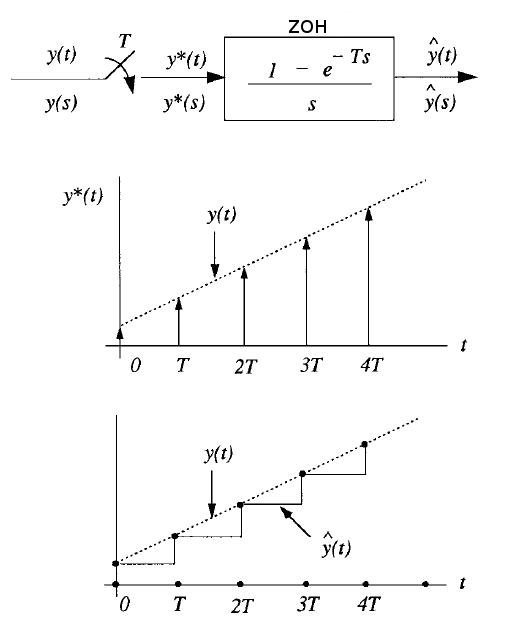
\includegraphics[scale=0.65]{referencial/img/zoh_wie_p155}
  \end{center}
  \fonte{Adaptado de \citeonline{BongWie2001}.} 
  \label{fig:zoh_wie_p155}
\end{figure}

Onde y(t) é o sinal que está sendo amostrado, y*(t) é o trem de pulsos amostrados e $\hat{y}(t)$ é o sinal resultante. Um ZOH ideal pode ser representando da seguinte forma:

\begin{equation}
  \hat{y}(s) \approx \frac{1-e^{-Ts}}{Ts}y(s)
\end{equation}

Essa expressão é de suma importância para a aquisição das variáveis que queremos controlar usando técnicas digitais.


%%%%%%%%%%%%%%%%%%%%%%%%%%%%%%%%%%%

\subsubsection{Controlador PID Digital}

Agora, desejamos descrever a representação do controlador PID da equação \ref{eq:PID} de forma discreta, para isso devemos usar a aproximação de Euler:

\begin{equation}
  s = \frac{1-z^{-1}}{T}
\end{equation}

Conseguimos expressar o controlador PID no domínio z da seguinte forma:

\begin{equation}
  u(t) = -K\left[1 + \frac{1}{T_i}\frac{T}{1-z^{-1}} + T_d\frac{1-z^{-1}}{T} \right]e(t)
\end{equation}

Com isso, podemos representar de forma discreta o controlador PID, isso pode ser visto na equação da sequência:

\begin{equation}\label{eq:pid_equation}
  u(t) = -K_p\left[y[k]-\frac{1}{T_i}{\hat{u}[k]}-T_d\frac{y[k]-y[k-1]}{T}\right]
\end{equation}

Onde

\begin{equation}
  \hat{u}[k] = \hat{u}[k-1] +Ty[k]
\end{equation}

Desse modo, concluímos a modelagem de um controlador PID, com um conjunto de equações que podem ser, de forma simples, implementadas em um sistema digital.


%%%%%%%%%%%%%%%%%%%%%%%%%%%%%%%%%%%

\subsubsection{Filtro de Kalman}

Quando se trabalha na aquisição de grandezas físicas, encontramos ruídos nos sinais amostrados. Esses ruídos podem inviabilizar o controle de uma planta, pois não informam o verdadeiro estado do sinal amostrado, fazendo com que o atuador atue de forma equivocada, levando a instabilidade o sistema. Uma forma de minimizar esse efeito, é utilizando o filtro de Kalman.

Filtro de Kalman é um algoritmo usado para estimar estados de variáveis de um sistema, sujeito a ruídos estocásticos. Esse algoritmo relaciona as informações sobre a dinâmica da planta e informações sobre o comportamento estocástico do dos sinais para estimar variáveis de estados da planta \cite{Levine1996}. Na figura \ref{fig:kalman_levine_p591}, temos a representação em diagrama de blocos do filtro de Kalman.

\begin{figure}[H]
  \caption{Diagrama de blocos do filtro de Kalman.}
  \begin{center}
      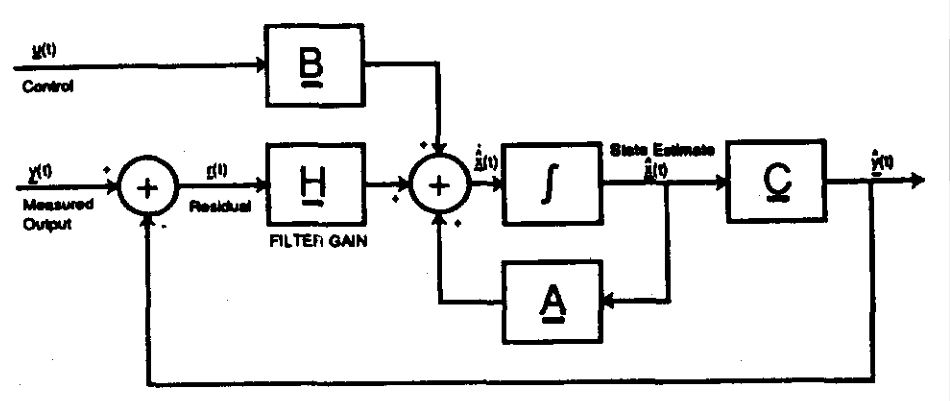
\includegraphics[scale=0.5]{referencial/img/kalman_levine_p591}
  \end{center}
  \fonte{Adaptado de \citeonline{Levine1996}.} 
  \label{fig:kalman_levine_p591}
\end{figure}

Onde $u(t)$ é o sinal do controlador, $y(t)$ é o sinal amostrado da saída da planta, $\hat {y}(t) $ é a saída estimada, H é o ganho do filtro e A, B e C são as matrizes em espaço de estados da dinâmica da planta.


%%%%%%%%%%%%%%%%%%%%%%%%%%%%%%%%%%%%%%%%%%%%%%%%%%%%%%%%%%%%%%%%%%%%%%

\section{Sintonia de Controladores}

Como podemos ver no modelo matemático e gráfico dos controladores PID, os valores de ajuste $K_p$, $T_i$ e $T_d$  podem assumir infinitos valores, sendo necessário a escolha do melhor conjunto desses valores para que a planta desempenhe o comportamento esperado \cite{Ogata}.


%%%%%%%%%%%%%%%%%%%%%%%%%%%%%%%%%%%

\subsection{Método de sintonia de Ziegler-Nichols}

Dois métodos clássicos de sintonia foram desenvolvidos em 1942 por Ziegler e Nichols. Esses dois métodos são baseados em características da resposta ao degrau e com a resposta em frequência. Na figura \ref{fig:ziegler-nichols_astrom_p135} podemos ver a resposta ao degrau e os parâmetros de atraso (L) e velocidade da resposta (a), que são usados para o cálculos dos parâmetros do controlador  \cite{Astrom1995}. 

\begin{figure}[H]
  \caption{Resposta ao degrau e seus parâmetros.}
  \begin{center}
      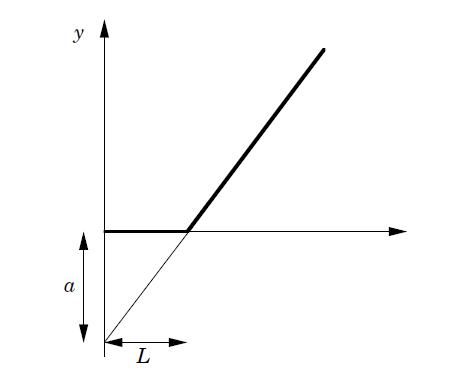
\includegraphics[scale=0.75]{referencial/img/ziegler-nichols_astrom_p135}
  \end{center}
  \fonte{\citeonline{Astrom1995}.} 
  \label{fig:ziegler-nichols_astrom_p135}
\end{figure}

Na tabela \ref{tab:Ziegler-Nichols} podemos ver as relações dos parâmetros $K_p$, $T_i$, $T_d$ e $T_p$ com os vistos na figura \ref{fig:ziegler-nichols_astrom_p135}. O outro método de se estimar os valores do controlador, é através de duas características da resposta em frequência: uma delas que é o ganho que deixa o sistema marginalmente estável ($K_u$), e a outra, é o período do sinal de referência que deixa o sistema marginalmente estável ($T_u$). Podemos ver na tabela \ref{tab:Ziegler-Nichols-freq} as relações entre $K_p$, $T_i$, $T_d$, $T_p$ e ($K_u$) e ($T_u$).

\begin{table}
  \caption{Parâmetros PID pelo método de Ziegler-Nichols - resposta ao degrau}
  \label{tab:Ziegler-Nichols}
  \centering%
  \begin{minipage}{.42\textwidth}
    \begin{tabular*}{\textwidth}{lllll}
      \hline
      {Controlador} & {K} & {$T_i$} & {$T_d$}& {$T_p$}\\ \hline
      \hline
      P    &  1/a   &     &      & 4L  \\ 
      PI   &  0.9/a & 3L  &      & 5.7L  \\
      PID  &  1.2/a & 2L  & L/2  & 3.4L  \\ \hline
    \end{tabular*}
    \fonte{Adaptado de \citeonline{Astrom1995}}
  \end{minipage}
\end{table}


\begin{table}
  \caption{Parâmetros PID pelo método de Ziegler-Nichols - resposta em frequência}
  \label{tab:Ziegler-Nichols-freq}
  \centering%
  \begin{minipage}{.52\textwidth}
    \begin{tabular*}{\textwidth}{lllll}
      \hline
      {Controlador} & {K} & {$T_i$} & {$T_d$}& {$T_p$}\\ \hline
      \hline
      P    &  0.5$K_u$   &           &             & $T_u$  \\ 
      PI   &  0.4$K_u$   & 0.8$T_u$  &             & 1.4$T_u$ \\
      PID  &  0.6$K_u$   & 0.5$T_u$  & 0.125$T_u$  & 0.85$T_u$  \\ \hline
    \end{tabular*}
    \fonte{Adaptado de \citeonline{Astrom1995}}
  \end{minipage}
\end{table}


%%%%%%%%%%%%%%%%%%%%%%%%%%%%%%%%%%%%%%%%%%%%%%%%%%%%%%%%%%%%%%%%%%%%%%

\subsection{Sintonia Automática de Controladores}

Como muitos sistemas sofrem variações temporais, distúrbios e o interesse do usuário em modificar constantemente a resposta da planta, cria-se a necessidade de automatizar o processo de sintonia, ao um simples comando do usuário. Além da simplicidade do conceito de implementação, os controladores PID são muito utilizados pela possibilidade de auto sintonia e adaptatividade dos controladores, pois a partir do comportamento da resposta ao degrau, podemos calcular os parâmetros do controlador e aplicarmos sem a intervenção humana\cite{Astrom1995}. Na figura \ref{fig:escolha_controle_astrom_p236}, podemos a partir do comportamento da planta, escolher a ou as técnicas mais adequadas que devemos implementar para controlar de forma satisfatória a planta.

\begin{figure}[H]
  \caption{Fluxograma para a escolha do método de sintonia.}
  \begin{center}
      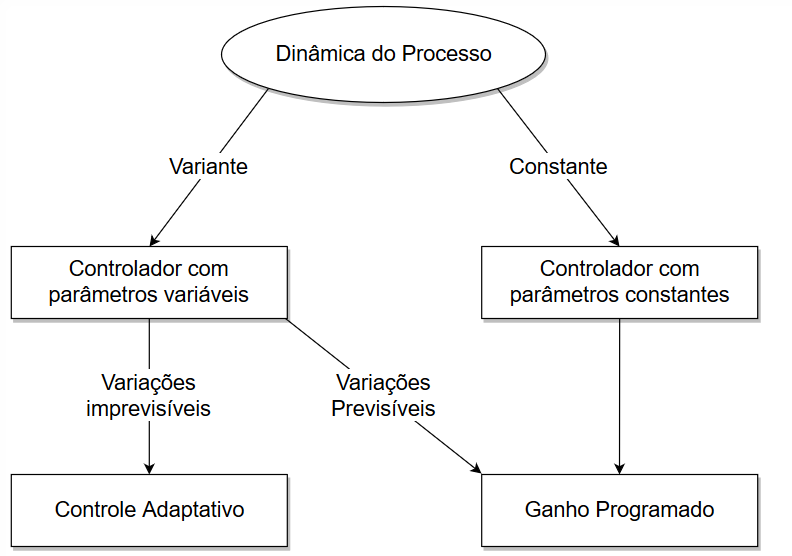
\includegraphics[scale=0.55]{referencial/img/escolha_controle_astrom_p236}
  \end{center}
  \fonte{Adaptado de \citeonline{Astrom1995}.} 
  \label{fig:escolha_controle_astrom_p236}
\end{figure}

Uma alternativa possível para sintonia de controladores, é o método do relé, ele, no modo clássico, se encontra entre os controladores com parâmetros constantes.


%%%%%%%%%%%%%%%%%%%%%%%%%%%%%%%%%%%

\subsubsection{Método do Relé}

Características da resposta em frequência podem ser descobertas se somarmos ao sinal de referência, uma onda retangular ao mesmo tempo em que o controlador PID está desconectado. Esse é o princípio do método de sintonia usando relé, onde o relé desempenha o papel do chaveamento e cria um sinal retangular sobreposto ao sinal de referência \cite{Levine1996}. Na imagem \ref{fig:pid_autotuning_relay_astrom_p239} podemos ver o conceito básico do método do relé. O modelo matemático usado para descrever o comportamento de um relé, pode ser visto na equação \ref{eq:n(a)} que está na sequência.
 
\begin{figure}[H]
  \caption{Modelo do método de auto sintonia via relé.}
  \begin{center}
      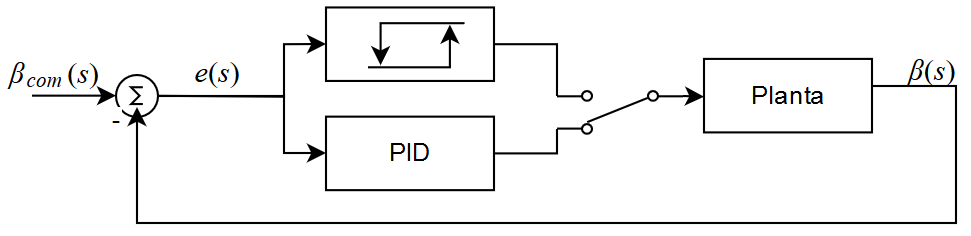
\includegraphics[scale=0.55]{referencial/img/pid_autotuning_relay_astrom_p239}
  \end{center}
  \fonte{Adaptado de \citeonline{Astrom1995}.} 
  \label{fig:pid_autotuning_relay_astrom_p239}
\end{figure}

\begin{equation}\label{eq:n(a)}
  N(a)=\frac{4d}{\pi a}\left(\sqrt{1-\left(\frac{\varepsilon}{a}\right)^{2}}-i\frac{\varepsilon}{a}\right) 
\end{equation}

Onde \textit{d} é a amplitude de oscilação do relé (normalmente até 10\% do sinal de referência), \textit{$\varepsilon$} é a histerese do relé e \textit{$a_r$} é a amplitude do sinal de referencia \cite{Levine1996}. Com isso, podemos calcular os parâmetros intermediários para a sintonia do controlador da seguinte forma:

\begin{equation}
  K_u \approx \frac{4d}{\pi a_r}
\end{equation}

Onde $T_u$ é o período de oscilação do sinal de interesse. Munido desses valores, podemos recorrer a tabela do método Ziegler-Nichols em resposta em frequência (Tabela \ref{tab:Ziegler-Nichols-freq}).


%%%%%%%%%%%%%%%%%%%%%%%%%%%%%%%%%%%%%%%%%%%%%%%%%%%%%%%%%%%%%%%%%%%%%%

\section{Estado da Arte - Controladores Inteligentes}

O estado da arte dentro de controle, está na criação de controladores inteligentes. Controle inteligente implementa conceitos de inteligência de organismos biológicos em forma de algoritmos. Esses algoritmos são usados para automatizar os processos de sintonia, promover a adaptação do controle perante as mudanças que a planta possa apresentar ou otimizar os parâmetros atuais. As duas principais formas de controle inteligente utilizadas na atualidade, são a por \textit{algoritmos genéticos} e \textit{por redes neurais}, onde a por redes neurais será explicada na sequência.


%%%%%%%%%%%%%%%%%%%%%%%%%%%%%%%%%%%

\subsection{Controle com Redes Neurais Artificiais}  %control hand p1017

Uma \textit{Rede Neural} (RNA) é um modelo matemático generalizado da cognição humana ou de um organismo biológico. O elemento básico de uma RNA é o neurônio, que associado em camada, forma uma rede de neurônios. Um neurônio pode ter n entradas e p saídas, e dentro de uma mesma camada, todos os neurônios devem ser idênticos. O processo de cognição é caracterizado como um comportamento não-linear, a função ($f_{rn}$) que descreve a excitação um neurônio binário unipolar,  pode ser vista na sequência \cite{Unal2013}. 

\begin{equation} \label{eq:neuron}
f(rn) \equiv \frac{1}{1+e^{-\lambda_n}}
\end{equation}

também

\begin{equation}
f(rn) \equiv sgn(rn) = \begin{Bmatrix}  1, \quad rn>0 \\ 1, \quad rn<0  \end{Bmatrix}
\end{equation}

Onde $\lambda_n$ é o ganho do neurônio. Uma representação gráfica de um neurônio natural comparado com um artificial pode ser visto na figura \ref{fig:neuronio_unal_p6}, onde os dendritos são representados pelas entradas $p_1, p_2, ..., p_R$, uma soma dessas entradas que posteriormente é aplicada a função da equação \ref{eq:neuron}, onde obtemos a saída $a$.

\begin{figure}[H]
  \caption{Célula de um neurônio natural e modelo matemático respectivo.}
    \begin{center}
        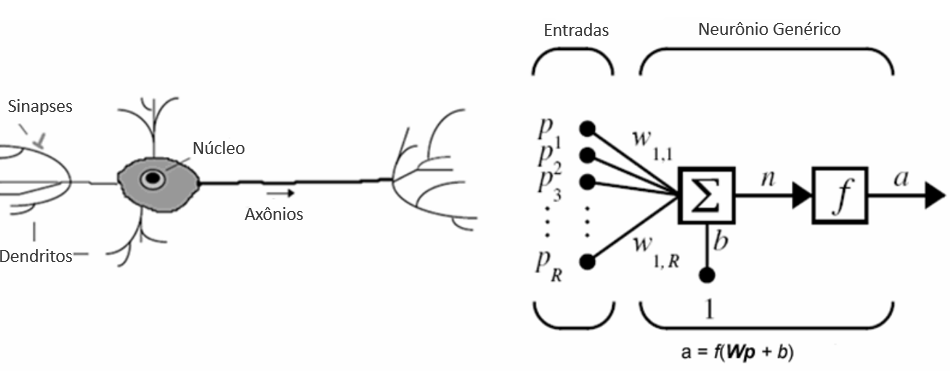
\includegraphics[scale=0.45]{referencial/img/neuronio_unal_p6}
  \end{center}
  \fonte{Adaptado de  \citeonline{Unal2013}.} 
  \label{fig:neuronio_unal_p6}
\end{figure}

Ao paralelizarmos um grupo de neurônios, criamos uma camada de neurônios, cada elemento dessa camada é conectado em todas as entradas, ou em todos os neurônios da camada anterior, ou posterior, ou ainda, nas saídas. Uma representação de uma rede neural pode ser vista na figura \ref{fig:feedforward_neural_astrom_p297}, onde temos 5 entradas ($u_1,...,u_5$) e duas saídas ($y_1 y_2$).

\begin{figure}[H]
  \caption{Representação de uma rede neural.}
  \begin{center}
      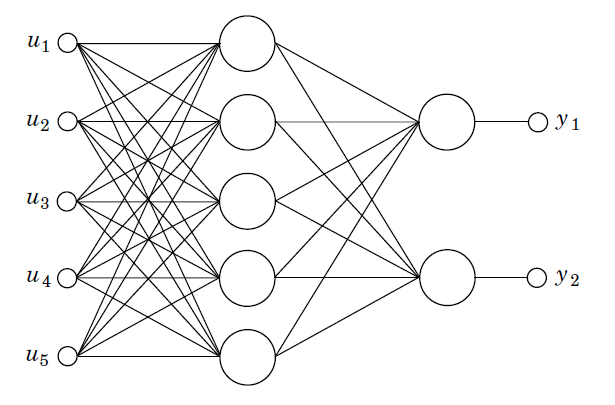
\includegraphics[scale=0.5]{referencial/img/feedforward_neural_astrom_p297}
  \end{center}
  \fonte{Adaptado de \citeonline{Astrom1995}.} 
  \label{fig:feedforward_neural_astrom_p297}
\end{figure}

Em controle, as RNAs são usadas principalmente em sistemas não lineares, onde existem regiões que a planta não é controlável pelas técnicas de controle clássicas \citeonline{Chen2004}. Nesse caso, a RNA recebe os sinais de controle do controlador e da saídas da planta, realiza as operações e encontra os novos parâmetros para o controlador PID. Um bom exemplo dessa topologia pode ser visto na figura \ref{fig:pid_neural_chen_p212}, onde os parâmetros obtidos pela rede neural ainda são linearizados para que sejam utilizados pelo controlador.

\begin{figure}[H]
  \caption{Controlador PID com rede neural.}
  \begin{center}
      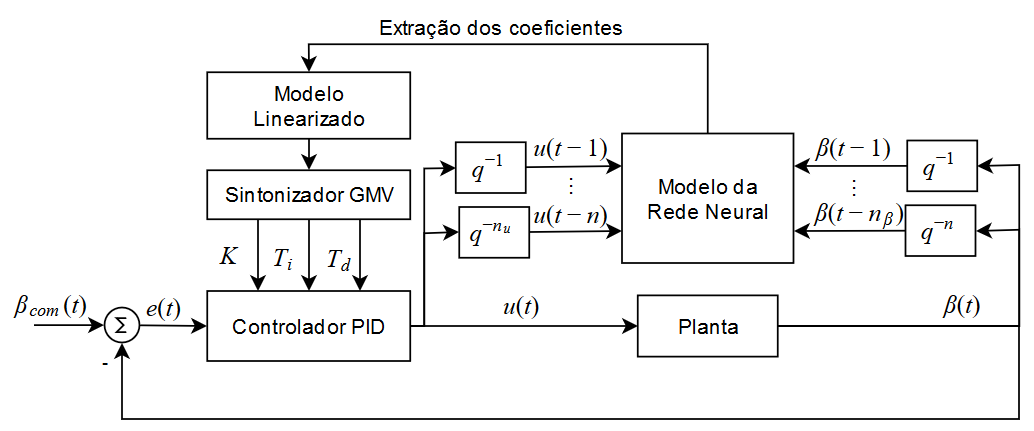
\includegraphics[scale=0.55]{referencial/img/pid_neural_chen_p212}
  \end{center}
  \fonte{Adaptado de \citeonline{Chen2004}.} 
  \label{fig:pid_neural_chen_p212}
\end{figure}

Na imagem anterior, existe o GMV (General Minimum Variance - Variância Mínima Geral) que é usado para extrair os parâmetros $K$ $T_i$ $T_d$ do modelo da rede neural linearizada \citeonline{Chen2004}.


%#########################

\subsubsection{Regressão Não-Linear Robusta}

Regressão é um método matemático para o ajuste de curva através da otimização de parâmetros que compõem a equação característica do sinal. O caso de interesse, é a regressão para sinais não-lineares, os quais são provenientes da RNA, que precisarão ser otimizados sobre a equação característica do controlador PID (equação \ref{eq:pid_equation}). De forma genérica, a equação que descreve um modelo não-linear pode ser descrita da seguinte forma \cite{robust2019}:

\begin{equation}
 y_i = f(x_i; \theta_e) + \epsilon_i, \quad\quad i = 1,...,n
\end{equation}

Onde $y_i$ é a resposta observável, $x_i$ é o vetor k-dimensional com os valores conhecidos e $\theta_e$ é p-dimensional com valores desconhecidos que influenciam a reposta observável e $\epsilon_i$ é o erro que satisfaz alguma regularidade estocástica. 

Um dos métodos mais usados para regressão, independente da linearidade do sistema, é o \textit{Método dos mínimos quadrados} (MMQ), que pode ser representado da seguinte forma:

\begin{equation}
 S(\theta_e) = \sum_{i=1}^{n}[y_i-f(x_i;\theta_e)]^2 
\end{equation}

Esse método por definição, é usado onde as amostras obedecem uma distribuição normal. Quando isso não é verdadeiro, usa-se o método MMQ robusto, onde o erro pode assumir outras distribuições mantando a boa resposta da regressão. Na figura \ref{fig:robust_regression}, podemos ver a comparação entre os métodos MMQ e MMQ Robusto, ficando clara a melhor resposta do MMQ Robusto.

\begin{figure}[H]
  \caption{Comparação entre os métodos de regressão não-lineares.}
  \begin{center}
      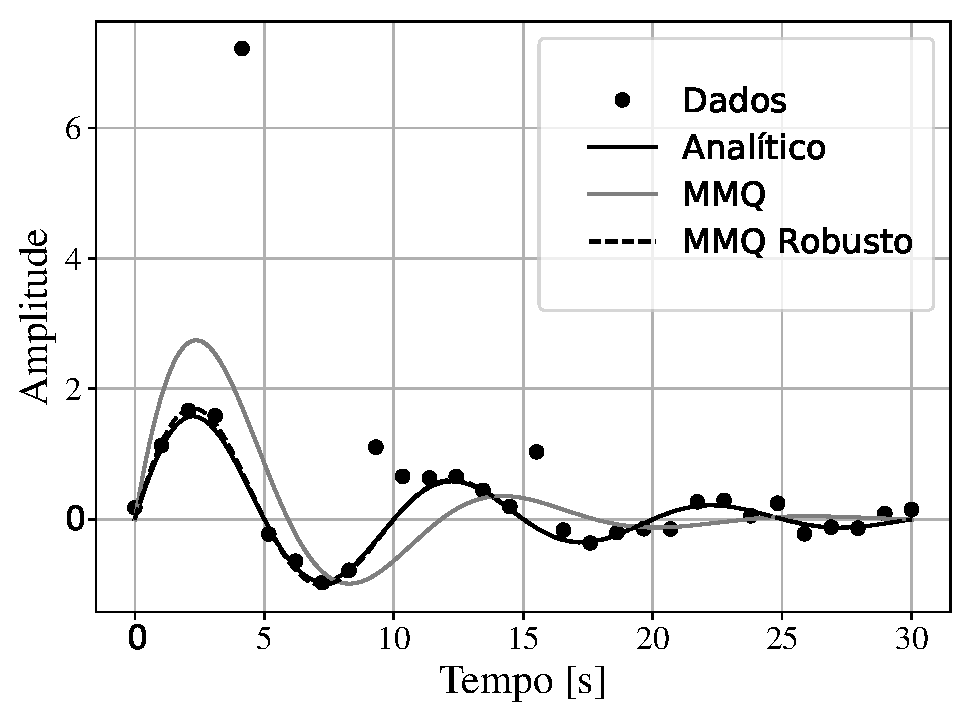
\includegraphics[scale=0.7]{referencial/img/robust_regression}
  \end{center}
  \fonte{Adaptado de \citeonline{RegressionPython}.} 
  \label{fig:robust_regression}
\end{figure}

Os últimos itens abordados, apontam algumas das modernas técnicas aplicadas em controle, as quais aplicarei no presente trabalho de forma conjunta, propondo uma técnica afim para a sintonia de controladores. Após elucidados os conceitos básicos para a realização do trabalho, todos os passos para a implementação da mecânica, do software e o sistema de controle serão descritos no próximo capítulo.